\section{Traditional Statistical models}

\subsection{ARIMA models}

\subsection{Exponential Smoothing models}

\subsection{Holt-Winters models}

\section{Machine Learning Methods}

\subsection{Bagging for Time Series}

According to \textcite{hastie2009} the bagging estimate is defined by

\begin{equation} 
\hat{f}_{bag}(x)=\frac{1}{B} \sum_{b=1}^B\hat{f}^{*b}(x)
\end{equation}

\noindent The bagging estimate is obtained by averaging the predictions $\hat{f}^{*b}(x)$ for\\ $ b=1,..,B $ from the statistical learning models fitted to a collection of B bootstrap samples obtained from the single training data set via taking repeated samples with replacement, i.e. bootstrapping.\\
Bagging is therefore a general-purpose technique for reducing the variance of a statistical learning method, which also increases that method's prediction accuracy \citep{james2013}.\\

\noindent The well-established bagging method was first introduced by \textcite{breiman1996} but it was not successfully applied in a time series forecasting context until 2016.\\
According to \textcite{petropoulos2018} the complication with time series consists in accounting for non-stationarity and autocorrelation in the bootstrapping procedure in order to produce bootstrapped samples that resemble the original data.\\
\textcite{bergmeir} propose a bootstrapping procedure for time series as illustrated in Figure \ref{fig: Bootstrapping procedure TS} that includes a Box-Cox transformation in order to stabilize the variance and a decomposition either in form of the loess method to extract trend and remainder in case of a non-seasonal time series or an STL decomposition in order to break the series down into the trend, seasonal and remainder components. 
The Box-Cox transformation, which was first introduced by \textcite{box1964}, is defined as follows:

\begin{equation}
	w_{t} =
	\begin{cases}
	log(y_{t}), & \lambda=0 \\
	(y_{t}^\lambda-1)/\lambda, & \lambda \neq0\\
	\end{cases}
\end{equation}

The optimal $\lambda \in [0,1]$ is chosen by dividing the series into subseries of length equal to the seasonality and minimzing the coefficient of variation $s/m^{(1-\lambda)}$ across those subseries, where $s$ stands for the standard deviation and $m$ for the sample mean of the subseries.
The authors then apply a bootstrapping method that allows for autocorrelation, the moving block bootstrap (MBB) as suggested by \textcite{kunsch1989}, to the extracted remainder of the series. In the next step, the series is reconstructed from its structural components, i.e. trend, seasonality, and the bootstrapped remainder. Finally, the Box-Cox transformation is inverted. The whole process is then repeated in order to obtain the bootstrapped series.\\ 


\begin{figure} [h]
\centering
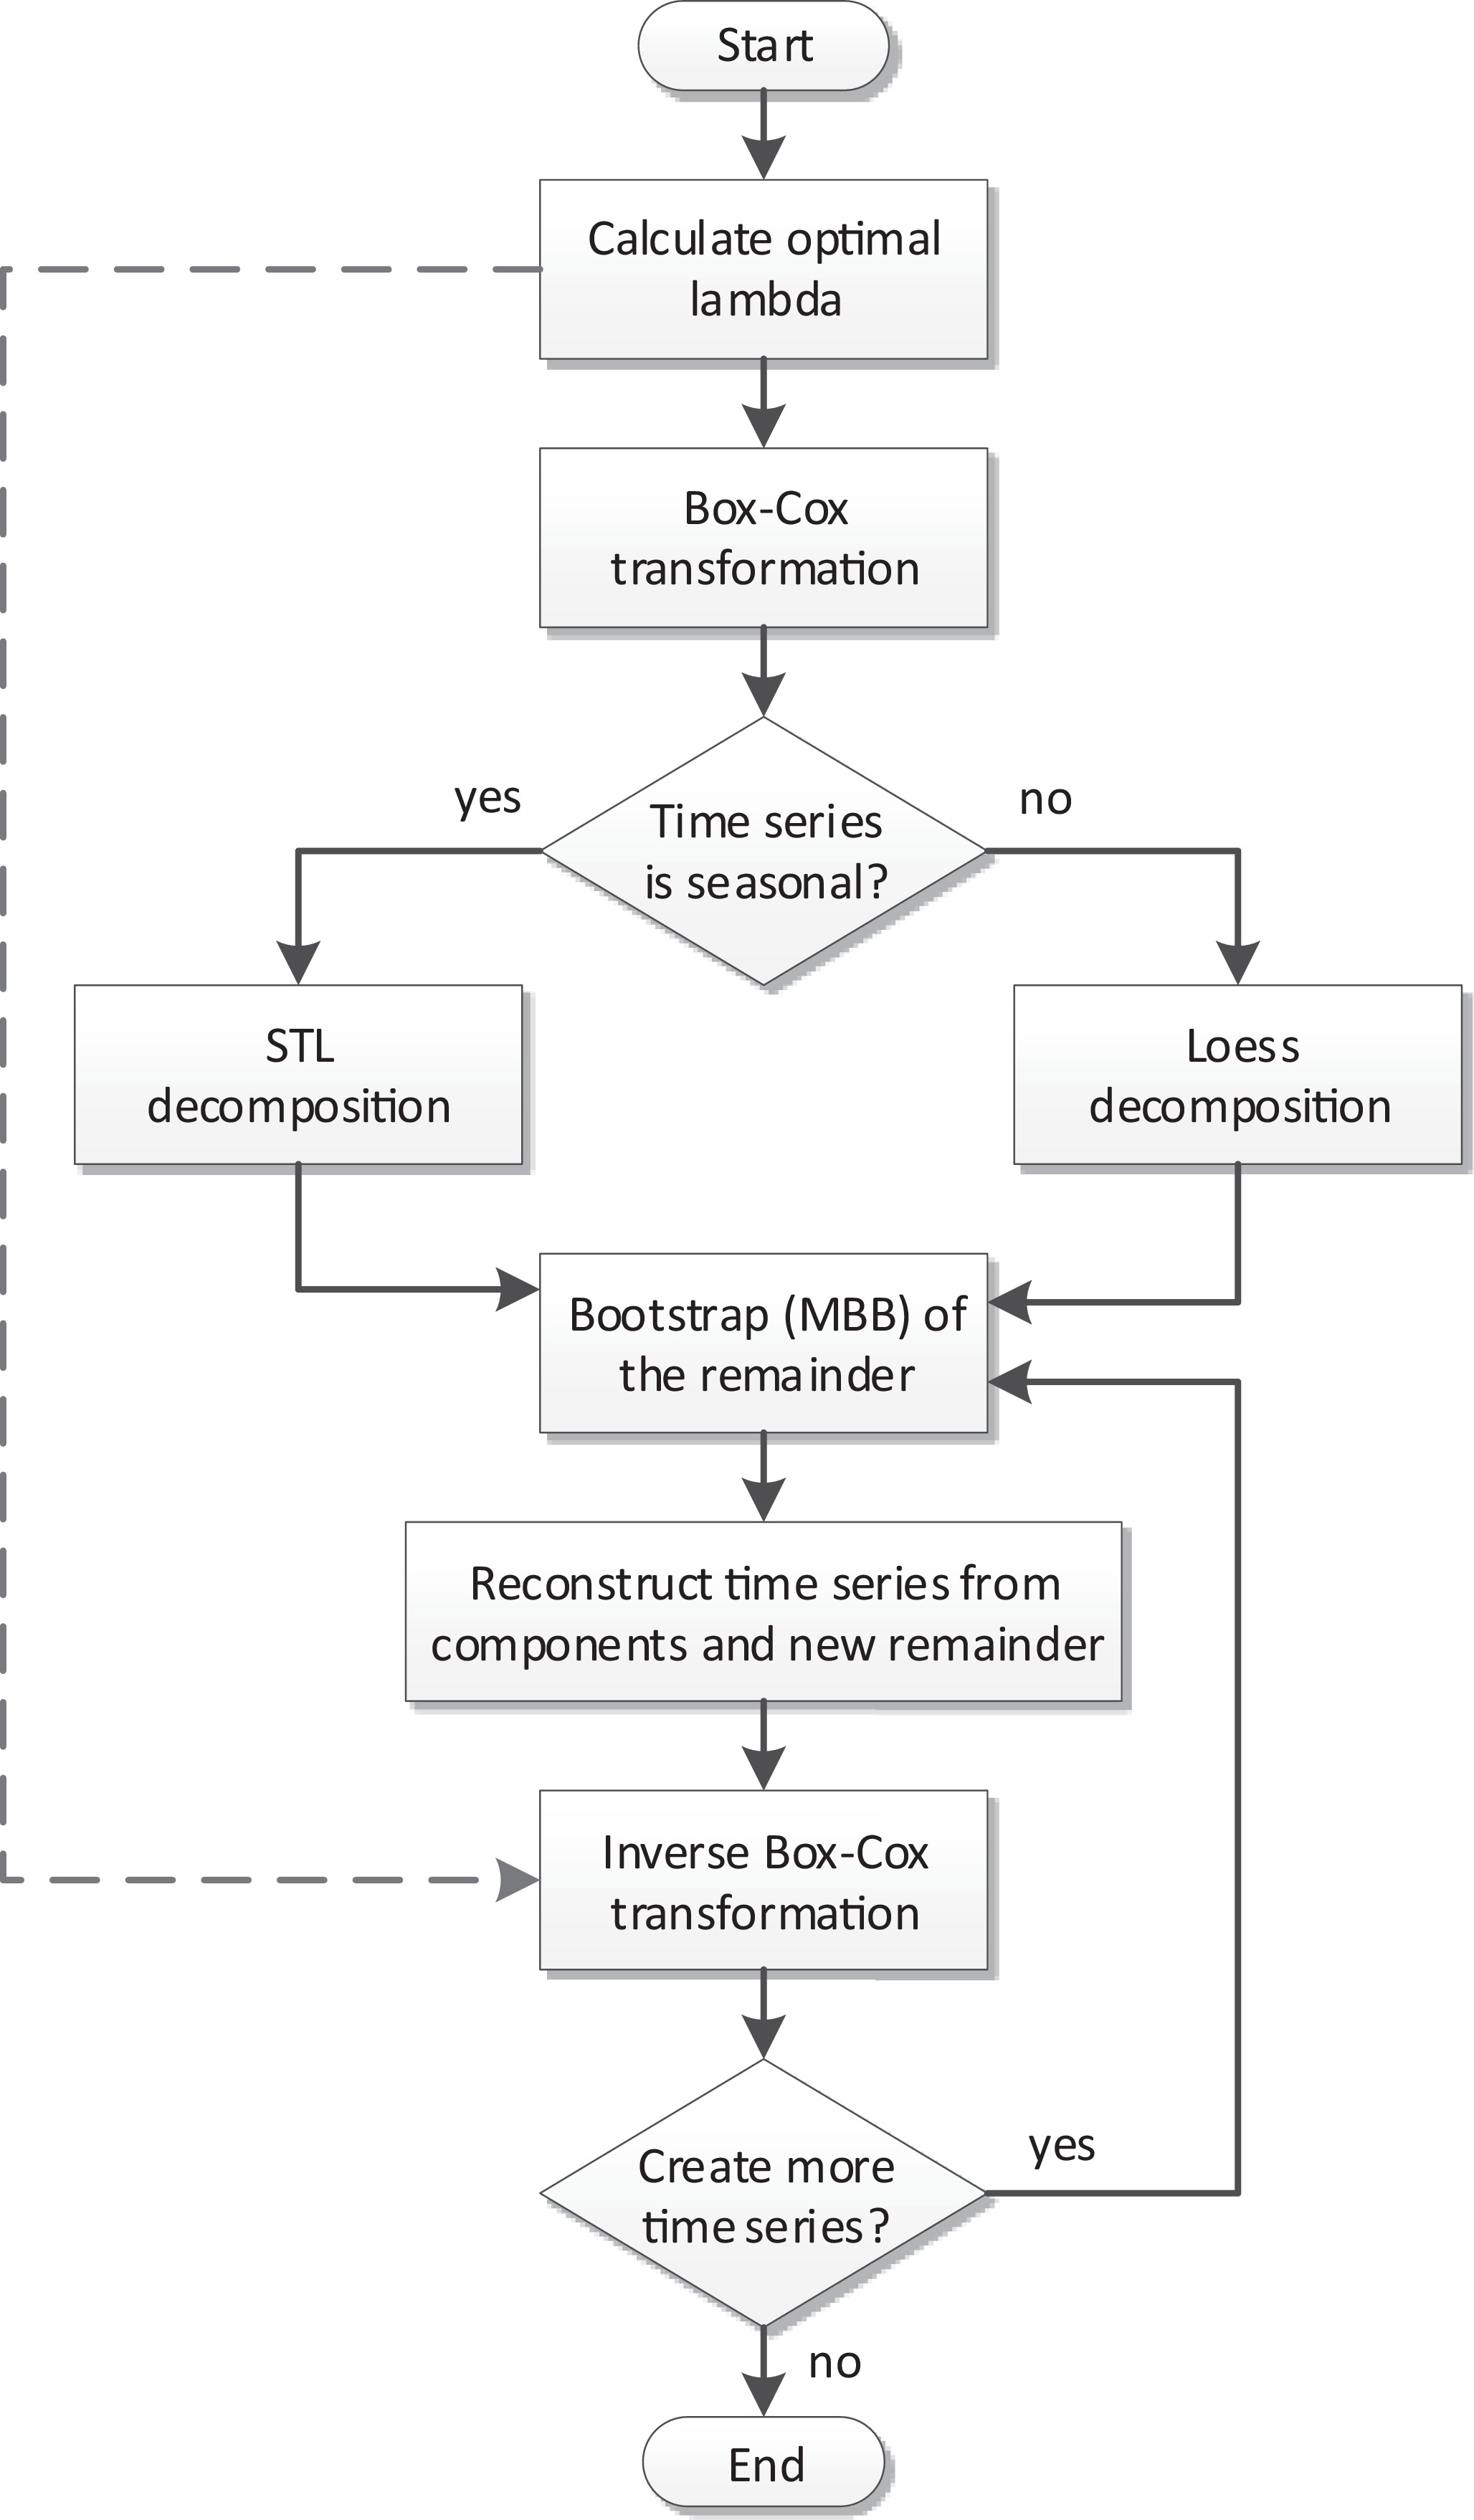
\includegraphics[scale=0.8]{TS}
\caption{Bootstrapping procedure for a time series (adapted from \textcite{petropoulos2018})}
\label{fig: Bootstrapping procedure TS}
\end{figure}

\textcite{bergmeir} find that the ensemble of bagged exponential smoothing models outperforms the regular exponential smoothing model consistently for monthly data on the M3 forecasting competition dataset, which is a common medium of comparison of newly introduced forecasting methods with existing state of the art models.


\subsection{Tree-based models for Time Series}

\textcite{galicia2019} propose a dynamic ensemble model for big data time series forecasting purposes as illustrated in Figure \ref{fig: Dynamic ensemble model} based on the three base models decision trees, random forests and gradient boosted trees. The ensemble weights are computed by weighted least squares assigning higher weights to more accurate ensemble members according to their past performance.\\

 
\noindent The authors found that the ensemble model outperformed the individual base models on a high sampling frequency dataset for the Spanish electricity market in terms of prediction accuracy as evidenced by lower mean absolute errors (MAE) and root mean squared errors (RMSE). Moreover, they found that the dynamic ensemble model could outperform Artificial Neural Network (ANN) and deep learning (DL) algorithms when evaluating forecast errors by yielding the lowest MAE and RMSE values on an Australia solar power dataset.

\begin{figure} [h]
\centering
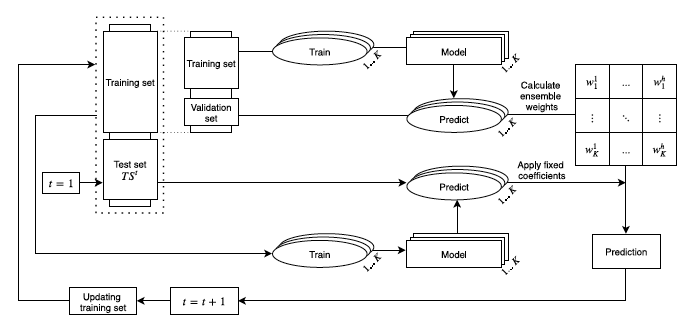
\includegraphics[scale=0.6]{ES}
\caption{Dynamic ensemble model (adapted from \textcite{galicia2019})}
\label{fig: Dynamic ensemble model}
\end{figure}

\subsection{Neural Network Models}